\chapter{Organização curricular do Curso}
\label{cap11}

O curso de Engenharia Eletrônica da UFPE segue as recomendações da Lei de Diretrizes e Bases da Educação Nacional (LDB – Lei 9.394 de 20/12/1996), o Projeto Político Pedagógico Institucional (PPPI, julho/2007), as Diretrizes Curriculares Nacionais do Curso de Graduação em Engenharia (Resolução CNE/CES nº 11/2002 de 11/03/2002), bem como a atual estruturação do Conjunto das Engenharias da UFPE.

Inicialmente, o aluno egresso do processo seletivo cursará o Ciclo Básico na Área II da Universidade. Para permitir ao aluno ter contato cedo com conteúdo profissional, e buscando contribuir para a diminuição da evasão, foi colocada a disciplina Introdução à Engenharia Elétrica no 1º período. Trata-se de encontros semanais onde o aluno é apresentado a conteúdo prático em laboratório de modo a motivar e despertar seu interesse pela eletrônica. Essa disciplina não tem avaliação, e o aluno é aprovado por frequência. 

A partir do 3º período, ele continuará as disciplinas do Ciclo Básico até o final do 4º período. Porém, iniciará, nessa ocasião, as disciplinas do Ciclo Profissional, tendo aulas expositivas dialogadas\footnote[6]{É uma exposição do conteúdo, com a participação ativa dos estudantes, cujo conhecimento prévio deve ser considerado e pode ser tomado como ponto de partida. O professor leva os estudantes a questionarem, interpretarem e discutirem o objeto de estudo, a partir do reconhecimento e do confronto com a realidade. Deve favorecer análise crítica, resultando na produção de novos conhecimentos. Propõe a superação da passividade e imobilidade intelectual dos estudantes. (ANASTASIOU, Léa das Graças Camargos; ALVES, Leonir Pessate (Org). Processos de Ensinagem na Universidade: pressupostos para estratégias de trabalho em aula. Joinville, SC: UNIVILLE, 2004, p. 79).} para o conteúdo teórico; e aulas práticas desenvolvidas nos laboratórios com auxílio de equipamentos de montagem de circuitos ou com uso de softwares. Essas disciplinas do Ciclo Profissional servirão para consolidar e estender os conhecimentos de matemática e ciências naturais visando a sua aplicação no âmbito do curso. Além disso, também a partir do 3º período, o aluno poderá iniciar a sua formação específica em Engenharia Eletrônica através de disciplinas eletivas, desde que tenha cursado todas as disciplinas pré-requisitos da eletiva desejada.

Do 5º ao 8º período, o aluno construirá os conhecimentos profissionais em engenharia básica, eletrônica analógica, eletrônica digital, controle e processamento de sinais que darão suporte aos conhecimentos específicos do curso. 

Do 8º ao 10º período, o aluno se aprofundará nos conhecimentos específicos do curso de Engenharia Eletrônica. Esses períodos são os mais indicados aos alunos cursarem as disciplinas eletivas, enquanto o curso oferece as disciplinas obrigatórias Segurança no Trabalho, Engenharia Econômica, Introdução ao Direito, Sociologia e Meio Ambiente e Administração. Tal momento de oferta foi escolhido, porque percebeu-se que essa seria a melhor ocasião, visto que somente ao final do curso é que o aluno adquire maturidade para entender a importância delas na preparação para o mercado de trabalho. No 10º período, o aluno realizará o Estágio Supervisionado (Lei 11788 de 2008, e escreverá seu Trabalho de Conclusão de Curso\footnote[7]{O aluno não é obrigado a cursar o Estágio Supervisionado ou TCC exatamente no 10º período, a colocação dessas disciplinas nesse período é apenas uma sugestão do curso.}. A disciplina TCC consiste em encontros com o professor-orientador durante todo o semestre, resultando na escolha, por parte do aluno, de um tema, geralmente interdisciplinar, para seu texto. O aluno será considerado aprovado no curso após completar a carga horária total e ter seu TCC aprovado pela banca examinadora.

É relevante mencionar que, ao longo dos diversos períodos do curso, serão transversalmente abordadas duas importantes questões: a étnico-racial e a ambiental. Com relação à primeira, o curso deve estimular os alunos a participar de atividades e iniciativas institucionais, como a realização de eventos e seminários, a distribuição de material didático e bibliográfico, abordando a problemática e as possíveis soluções; tais iniciativas devem se somar ao fato de a UFPE já destinar percentual de cotas para negros e pardos por ocasião do ingresso em seus cursos. Além disso, essa questão será abordada especificamente em disciplinas de conteúdo humanístico e de ciências sociais, como CS100 - Sociologia e Meio-ambiente e PG300 - Introdução ao Direito, como também nos instrumentos de avaliação para identificação de problemas entre discente-discente, discente-docente ou docente-docente.

A questão ambiental também é abordada no conteúdo das disciplinas de forma interdisciplinar em Engenharia Eletrônica através da conscientização para a necessidade do desenvolvimento e da adoção de tecnologias “verdes”, ou seja, de baixo consumo de energia nos dispositivos e sistemas eletrônicos. Isso será feito em diversas disciplinas ao longo do curso. Em particular, as disciplinas CS100 - Sociologia e Meio Ambiente, ES232 - Introdução aos Dispositivos Semicondutores dão foco especial aos riscos ambientais das tecnologias envolvidas na fabricação de produtos eletrônicos e ao tratamento adequado para os resíduos dessa produção.

O curso de Engenharia Eletrônica opera no período diurno, nos turnos da manhã e tarde. A carga horária total do curso é de 3.600 horas e pode ser concluída em um mínimo de 8 semestres e no máximo de 20 semestres. O número de vagas ofertadas é de 20 alunos por semestre no turno manhã/tarde (20 na 1ª entrada e 20 na 2ª entrada).

A carga horária do curso está distribuída com os seguintes componentes:
\begin{enumerate}
\item[I)] Disciplinas obrigatórias do ciclo básico das engenharias da UFPE (1050 horas);
\item[II)] Disciplinas obrigatórias do ciclo profissional do Curso (1890 horas);
\item[III)] Componentes eletivos do perfil (240 horas);
\item[IV)] Componentes eletivos livres (60 horas)
\item[V)] Atividades Complementares (120 horas)
\item[VI)] Trabalho de Conclusão de Curso (60 horas)
\item[VII)] Estágio Curricular (180 horas)
\end{enumerate}

Em relação ao que determina as Diretrizes Curriculares Nacionais do Curso de Graduação em Engenharia, RESOLUÇÃO CNE/CES 11, DE 11 DE MARÇO DE 2002, tem-se:

\begin{table}[h!]
	\caption{Distribuição da carga horária}
	\centering
	\resizebox{0.7\textwidth}{!}{
		\begin{tabular}{|c|c|c|}
			\hline
			Núcleo de Conteúdos básicos (mínimo de 30\%) &   1450 h  &  40,27\%  \\ \hline
			Núcleo de Conteúdos Profissionalizantes (mínimo de 15\%) &  1115 h   & 30,97\%   \\ \hline
		Núcleo de Conteúdos Específicos		& 1035 h    & 28,75\%   \\ \hline
		
	\end{tabular}}\\
%	{\footnotesize Fonte: O Autor(2023).}
	\label{tab1}
\end{table}

O curso de Engenharia Eletrônica da UFPE tem um perfil de formação determinado pelas disciplinas da sua matriz curricular, descrita abaixo, com área de concentração única em eletrônica, sem ênfases ou habilitações específicas. Estas disciplinas encontram-se distribuídas em dez períodos, e obedecem a restrições de pré-requisitos e co-requisitos. Desta forma, pode-se representá-las graficamente para mostrar estas dependências, por meio das tabelas e figuras a seguir.

\begin{figure}[h!]
	\caption{Disciplinas por período.}
	\begin{center}
		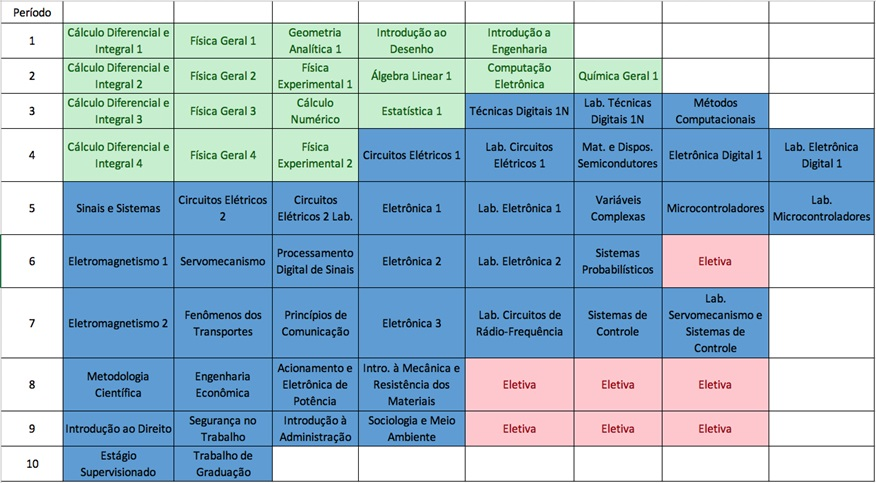
\includegraphics[width=7cm]{Ilustrações/Figura 01.jpg}\\
		{\footnotesize Fonte: Os autores.}
		\label{3.2b.eps}
	\end{center}
\end{figure}

\begin{figure}[h!]
	\caption{Disciplinas Eletivas.}
	\begin{center}
		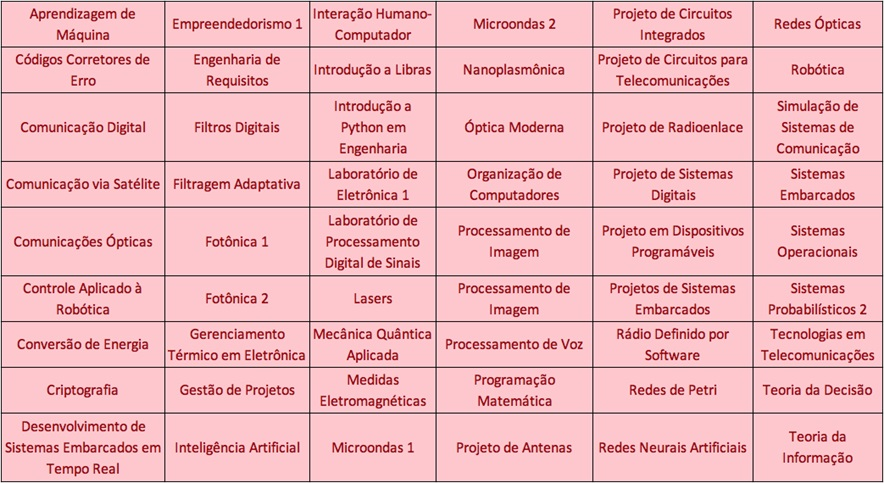
\includegraphics[width=7cm]{Ilustrações/Figura 02.jpg}\\
		{\footnotesize Fonte: Os autores.}
		\label{3.2b.eps}
	\end{center}
\end{figure}

\begin{figure}[h!]
	\caption{Organização da estrutura curricular do perfil 4507 de Engenharia Eletrônica.}
	\begin{center}
		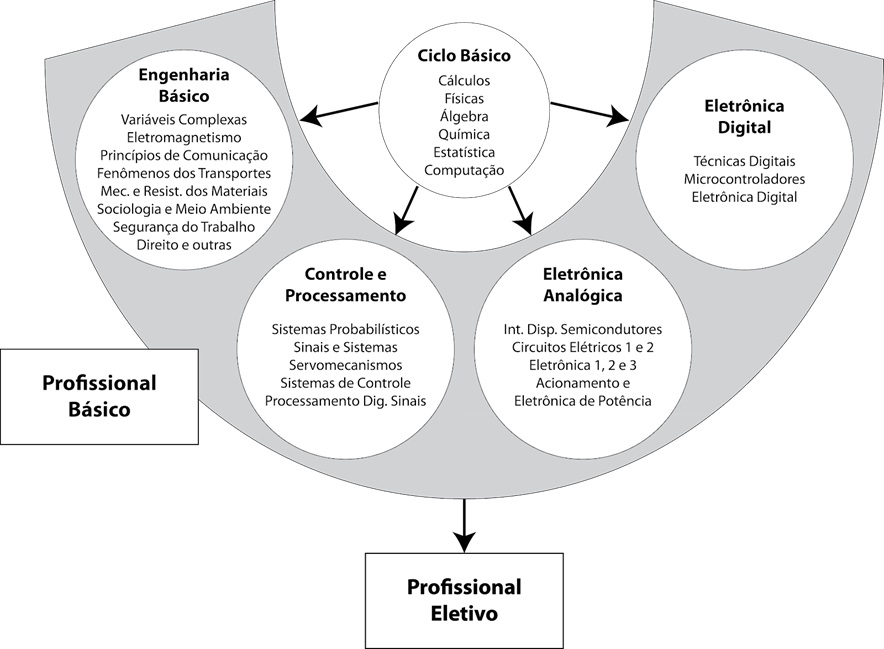
\includegraphics[width=7cm]{Ilustrações/Figura 03.jpg}\\
		{\footnotesize Fonte: Os autores.}
		\label{3.2b.eps}
	\end{center}
\end{figure}

\begin{figure}[h!]
	\caption{Disciplinas obrigatórias do ciclo profissional e suas interdependências (perfil 4507 de Engenharia Eletrônica).}
	\begin{center}
		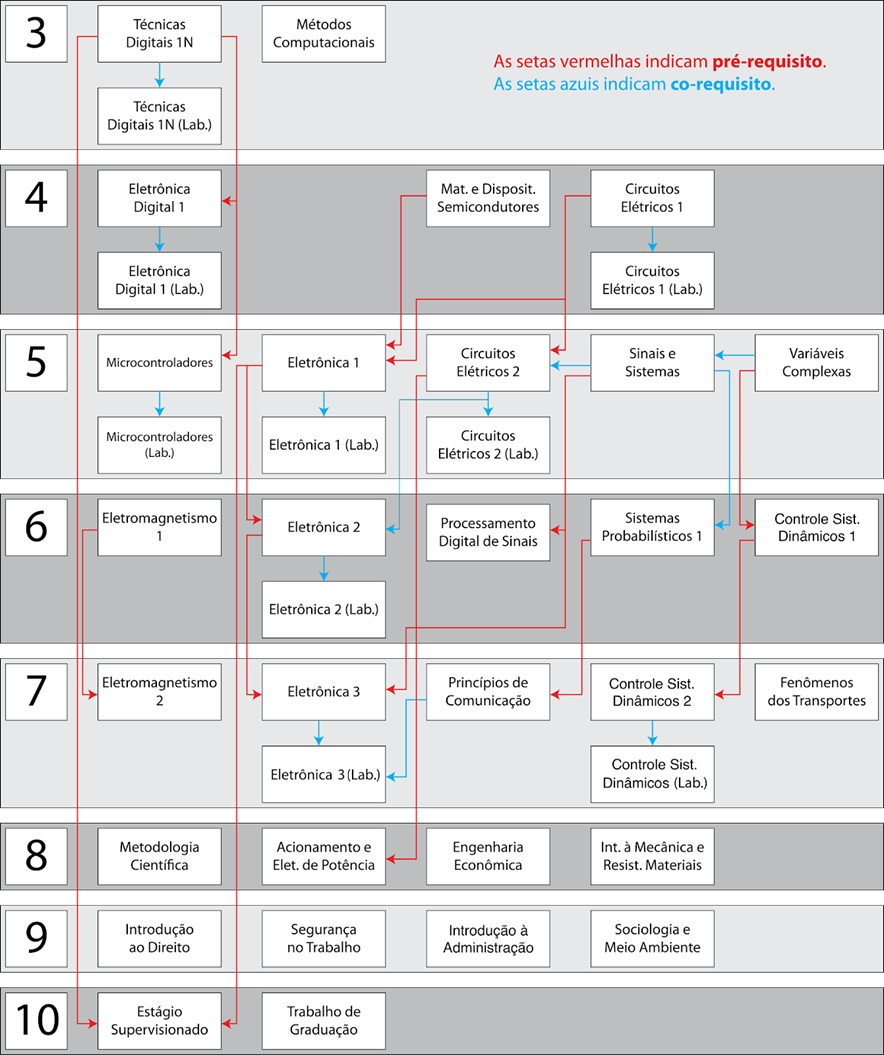
\includegraphics[width=7cm]{Ilustrações/Figura 04.jpg}\\
		{\footnotesize Fonte: Os autores.}
		\label{3.2b.eps}
	\end{center}
\end{figure}